\documentclass[11pt,a4paper]{article}
\usepackage[utf8]{inputenc}
\usepackage[portuguese]{babel}
\usepackage[T1]{fontenc}
\usepackage{amsmath}
\usepackage{graphicx}
\usepackage{amsfonts}
\usepackage{amssymb}
\usepackage{float}
\usepackage{indentfirst}
\usepackage[left=2.5cm,right=2.5cm,top=2.5cm,bottom=2.5cm]{geometry}
\author{Murilo Camargos}
\begin{document}

\begin{minipage}[t]{.3\textwidth}
\vspace{-20pt}
\begin{figure}[H]

\includegraphics[scale=0.5]{unimontes.png}
\end{figure}
\end{minipage}% <---------------- Note the use of "%"
\begin{minipage}[t]{.7\textwidth}
\textsc{\large Universidade Estadual de Montes Claros}
\vspace{0.25cm}\hrule\vspace{0.25cm}
Centro de Ciências Exatas e Tecnológicas - CCET\\[0.08cm]
Departamento de Ciências da Computação - DCC\\[0.08cm]
Engenharia de Sistemas - 6º Período
\end{minipage}

\vspace*{\fill}
\begin{center}
\bf
Murilo Cesar Osorio\\
\vspace*{\fill}
\Huge
TP1: Algoritmos Genéticos
\end{center}
\vspace*{\fill}
\begin{minipage}[t]{.6\textwidth}
\hspace{1pt}
\end{minipage}% <---------------- Note the use of "%"
\begin{minipage}[t]{.4\textwidth}
Trabalho apresentado ao Professor \mbox{João Batista Mendes} da disciplina Computação Evolutiva do 6º período do curso de Engenharia de Sistemas.
\end{minipage}

\thispagestyle{empty}
\vspace*{\fill}
\begin{center}
Montes Claros - MG\\
Fevereiro de 2017
\end{center}
\newpage


\section{Introdução}
O trabalho consiste na utilização de algoritmos genéticos e seus operadores para resolução de um problema do tipo caixa preta cuja função de saída é dada pela Equação \ref{ysaida}. A representação do problema é binária e as soluções candidatas possuem 36 bits, $b_{1}$ corresponde ao primeiro, ao passo que $b_{36}$ corresponde ao último bit da \textit{string}.

\begin{equation}
\begin{array}{rl}
y_{saida}=&9+b_{2}b_{5}-b_{23}b_{14}+b_{24}b_{4}-b_{21}b_{10}+b_{36}b_{15}-b_{11}b_{26}+b_{16}b_{17}\\
&+b_{3}b_{33}+b_{28}b_{19}+b_{12}b_{34}-b_{31}b_{32}-b_{22}b_{25}+b_{35}b_{27}-b_{29}b_{7}\\
&+b_{8}b_{13}-b_{6}b_{9}+b_{18}b_{20}-b_{1}b_{30}+b_{23}b_{4}+b_{21}b_{15}+b_{26}b_{16}\\
&+b_{31}b_{12}+b_{25}b_{19}+b_{7}b_{8}+b_{9}b_{18}+b_{1}b_{33}
\end{array}
\label{ysaida}
\end{equation}

É possível perceber, levando a zero os termos que são subtraídos e a um os que são somados, que o valor máximo da Equação \ref{ysaida} é \textbf{27}. Portanto, vinte e sete corresponde ao \textit{fitness} ótimo para este problema.

\section{Objetivos}
Os objetivos deste trabalho são de aprender os conceitos que permeiam o tópico de estudos de Algoritmos Genéticos através da implementação de seus operadores e algumas variantes de cada um deles. Além disso, por ter um estudo estatístico envolvido, o trabalho permite que o aluno possa aprender via gráficos as nuances do dimensionamento de um algoritmo genético, no que diz respeito ao seu comportamento de acordo com a escolha dos operadores, população inicial, taxas de mutação e cruzamento, e diversos outros parâmetros ajustáveis.

\section{Materiais e Métodos}
O trabalho foi implementado utilizando a linguagem \textbf{Python 2.7} com auxílio da bibliotecas \textbf{Numpy} e \textbf{Matplotlib}. A modelagem foi feita utilizando conceitos de orientação a objetos por tornar mais fácil a compreensão do código e deixar mais claro o encapsulamento dos métodos e atributos.

Foram criadas duas classes; a classe Pop modela uma população de tamanho $T$, dimensão $D$ e uma função de \textit{fitness}, os métodos dessa classe são os operadores de mutação, seleção, cruzamento e substituição; a segunda classe (GA) é responsável por processar o dicionário de configurações que o usuário pode informar e realizar os testes. O teste estatístico de Wilcoxon foi calculado utilizando a biblioteca \textbf{stats} do pacote \textbf{scipy}.

\subsection{Classe Pop}
Esta classe generaliza uma população com atributos de tamanho ($T$) e dimensão ($D$). A população é representada por uma matriz ($M$) \textit{np.array} com $N$ linhas (indivíduos) e $D$ colunas; o \textit{fitness} é definido pelo usuário como uma função que recebe uma linha dessa matriz e retorna um valor que determina a qualidade da solução.

Os métodos representados por esta classe são:
\begin{enumerate}
	\item \textbf{eval}: recebe a matriz $M$ como entrada e retorna um vetor $F^{1\times N}$ com os valores de \textit{fitness} de cada solução.
	\item \textbf{selection}: realiza a operação de seleção na população $M$, usando o algoritmo de torneio binário ou roleta (a ser definido pelo usuário) e retorna uma nova população $S$.
	\item \textbf{crossover}: realiza a operação de cruzamento na população $S$, usando o algoritmo de cruzamento uniforme ou com um ponto de corte. Retorna uma nova população $C$.
	\item \textbf{mutation}: faz mutações na população $C$ com as metodologias bit-a-bit e uniforme. Retorna uma nova população $E$.
	\item \textbf{substitution}: faz a substituição da população $E$ na população $M$ inicial utilizando elitismo.
\end{enumerate}

\subsection{Classe GA}
Esta classe recebe as configurações do algoritmo fornecidas pelo usuário e realiza os testes, também determinados pelo usuário. Seu valor de inicialização é um dicionário com as seguintes chaves:
\begin{itemize}
\footnotesize
\setlength\itemsep{0em}
\item \textbf{popSize}: <inteiro> tamanho da população;
\item \textbf{popDim}: <inteiro> dimensão da população;
\item \textbf{representation}: <str> tipo de representação ['binary'];
\item \textbf{fitnessEval}: <object> uma função python para calculo de \textit{fitness};
\item \textbf{crossRate}: <float> taxa de cruzamento [0,1];
\item \textbf{crossType}: <str> tipo de cruzamento ['uniform', '1cp'];
\item \textbf{selectionType}: <str> tipo de seleção ['roulette','tournament'];
\item \textbf{mutationRate}: <float> taxa de mutação [0,1];
\item \textbf{mutationType}: <str> tipo de mutação ['uniform', '1bit'];
\item \textbf{maxEpochs}: <int> numero máximo de épocas.
\end{itemize}

Para realizar os testes, a função \textbf{test} implementa um GA geral e recebe como parâmetros a quantidade de testes a serem realizados com as configurações listadas anteriormente e o nome do arquivo que será salvo com os resultados. Cada um dos testes é inicializado com uma população aleatória; ao final do teste, o maior \textit{fitness} da população é inserido num vetor que será retornado ao final de todos os testes.

\section{Resultados e Discussões}
\subsection{Teste 1: Avaliação do efeito do tipo de cruzamento}
Os parâmetros para a realização deste teste foram: seleção por roleta, mutação bit a bit, cruzamentos uniforme e com um ponto de corte, taxa de cruzamento igual a 0.8, taxa de mutação igual a 0.025, número de indivíduos igual a 30 e limitada a 50 gerações. Pelos resultados abaixo, podemos perceber que a melhor configuração para o tipo de cruzamento é o uniforme.\\

\begin{minipage}{0.5\linewidth}
\textbf{Uniforme:}
\begin{itemize}
	\footnotesize
	\setlength\itemsep{0em}
	\item Número de sucessos: \textbf{54}
	\item Maior \textit{fitness}: \textbf{27}
	\item Menor \textit{fitness}: \textbf{25}
	\item Média dos \textit{fitness}: \textbf{26.52}
	\item Desvio padrão dos \textit{fitness}: \textbf{0.61}
\end{itemize}
\end{minipage}
\begin{minipage}{0.5\linewidth}
\textbf{Com um ponto de corte:}
\begin{itemize}
	\footnotesize
	\setlength\itemsep{0em}
	\item Número de sucessos: \textbf{0}
	\item Maior \textit{fitness}: \textbf{23}
	\item Menor \textit{fitness}: \textbf{19}
	\item Média dos \textit{fitness}: \textbf{21.12}
	\item Desvio padrão dos \textit{fitness}: \textbf{1}
\end{itemize}
\end{minipage}

\begin{minipage}{0.5\linewidth}
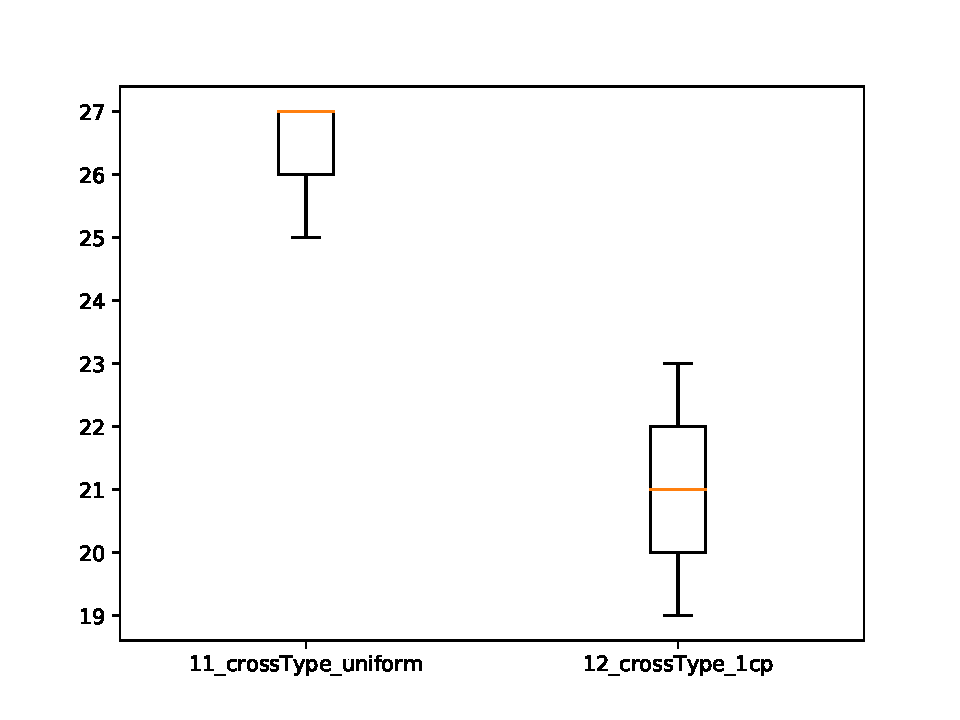
\includegraphics[scale=0.5]{teste1.pdf} 
\end{minipage}
\begin{minipage}{0.5\linewidth}
É visível, pelo \textit{boxplot}, que o primeiro método de cruzamento teve resultado melhor que o segundo. O teste de Wilcoxon resultou em \mbox{\textbf{2.52e-34}}, ou seja, os resultados são estatisticamente diferentes.
\end{minipage}

\subsection{Teste 2: Avaliação do efeito do tipo de seleção}
O teste de Wilcoxon para este resultado foi \textbf{1.34e-6}, indicando que a diferença entre os resultados foi pequena. De fato, a utilização do método da roleta ou do torneio binário não influenciaram muito no resultado, no entanto, o método da roleta foi ligeiramente melhor nos testes.\\

\begin{minipage}{0.25\linewidth}
\textbf{Roleta:}
\begin{itemize}
	\footnotesize
	\setlength\itemsep{0em}
	\item Sucessos: \textbf{58}
	\item Maior \textit{fitness}: \textbf{27}
	\item Menor \textit{fitness}: \textbf{25}
	\item $\mu_{\textit{fitness}}$: \textbf{26.52}
	\item $\sigma_{\textit{fitness}}$: \textbf{0.61}
\end{itemize}
\end{minipage}
\begin{minipage}{0.25\linewidth}
\textbf{Torneio:}
\begin{itemize}
	\footnotesize
	\setlength\itemsep{0em}
	\item Sucessos: \textbf{56}
	\item Maior \textit{fitness}: \textbf{27}
	\item Menor \textit{fitness}: \textbf{24}
	\item $\mu_{\textit{fitness}}$: \textbf{26.5}
	\item $\sigma_{\textit{fitness}}$: \textbf{0.63}
\end{itemize}
\end{minipage}
\begin{minipage}{0.4\linewidth}
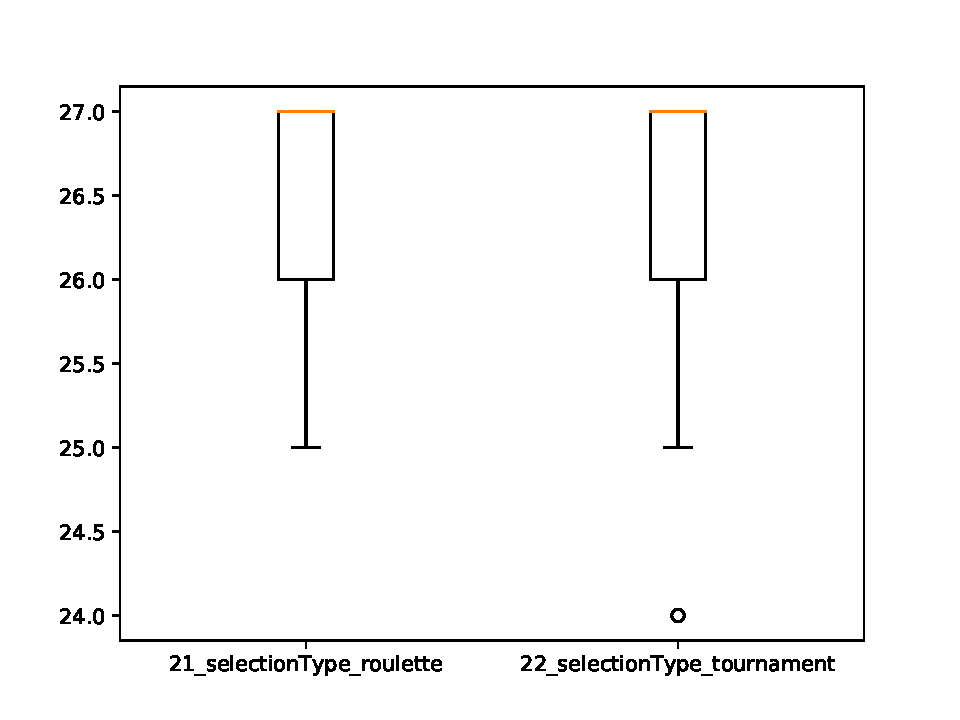
\includegraphics[scale=0.5]{teste2.pdf} 
\end{minipage}

\subsection{Teste 3: Avaliação do efeito do tipo de mutação}
O teste de Wilcoxon para este resultado foi \textbf{0.06}, indicando que a diferença entre os resultados foi pequena. De fato, a utilização do método da mutação uniforme ou bit-a-bit não influenciaram muito no resultado, no entanto, o método uniforme foi melhor nos testes no que diz respeito às piores e melhores soluções e na quantidade de sucessos. O \textit{boxplot} mostra os valores fora da curva, chamados \textit{outliars}.\\

\begin{minipage}{0.25\linewidth}
\textbf{Uniforme:}
\begin{itemize}
	\footnotesize
	\setlength\itemsep{0em}
	\item Sucessos: \textbf{58}
	\item Maior \textit{fitness}: \textbf{27}
	\item Menor \textit{fitness}: \textbf{25}
	\item $\mu_{\textit{fitness}}$: \textbf{26.52}
	\item $\sigma_{\textit{fitness}}$: \textbf{0.61}
\end{itemize}
\end{minipage}
\begin{minipage}{0.25\linewidth}
\textbf{Bit-a-bit:}
\begin{itemize}
	\footnotesize
	\setlength\itemsep{0em}
	\item Sucessos: \textbf{19}
	\item Maior \textit{fitness}: \textbf{27}
	\item Menor \textit{fitness}: \textbf{22}
	\item $\mu_{\textit{fitness}}$: \textbf{25.52}
	\item $\sigma_{\textit{fitness}}$: \textbf{1.14}
\end{itemize}
\end{minipage}
\begin{minipage}{0.4\linewidth}
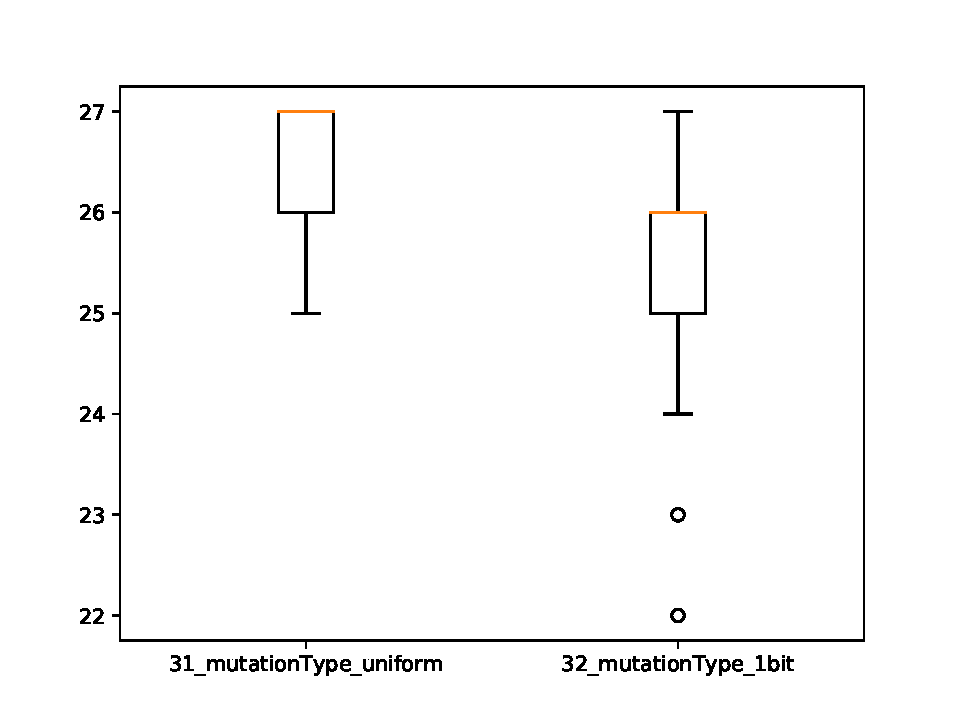
\includegraphics[scale=0.5]{teste3.pdf} 
\end{minipage}

\subsection{Teste 4: Avaliação do efeito da probabilidade de cruzamento}
Os valores para $P_C=0.8$ já foram mostrados anteriormente. Pode-se perceber que $P_C=0.8$ retorna os melhores resultados. Os valores do teste de Wilcoxon para as amostras ($P_C=0.2$, $P_C=0.5$), ($P_C=0.2$, $P_C=0.8$) e ($P_C=0.5$, $P_C=0.8$) são, respectivamente, \textbf{2.52e-34}, \textbf{2.52e-34} e \textbf{6.79e-31}; isto indica que os resultados são estatisticamente diferentes.\\

\begin{minipage}{0.25\linewidth}
\textbf{$P_C=0.2$}
\begin{itemize}
	\footnotesize
	\setlength\itemsep{0em}
	\item Sucessos: \textbf{0}
	\item Maior \textit{fitness}: \textbf{24}
	\item Menor \textit{fitness}: \textbf{19}
	\item $\mu_{\textit{fitness}}$: \textbf{20.95}
	\item $\sigma_{\textit{fitness}}$: \textbf{1.24}
\end{itemize}
\end{minipage}
\begin{minipage}{0.25\linewidth}
\textbf{$P_C=0.5$}
\begin{itemize}
	\footnotesize
	\setlength\itemsep{0em}
	\item Sucessos: \textbf{7}
	\item Maior \textit{fitness}: \textbf{27}
	\item Menor \textit{fitness}: \textbf{23}
	\item $\mu_{\textit{fitness}}$: \textbf{24.96}
	\item $\sigma_{\textit{fitness}}$: \textbf{1.09}
\end{itemize}
\end{minipage}
\begin{minipage}{0.4\linewidth}
\begin{minipage}{0.4\linewidth}
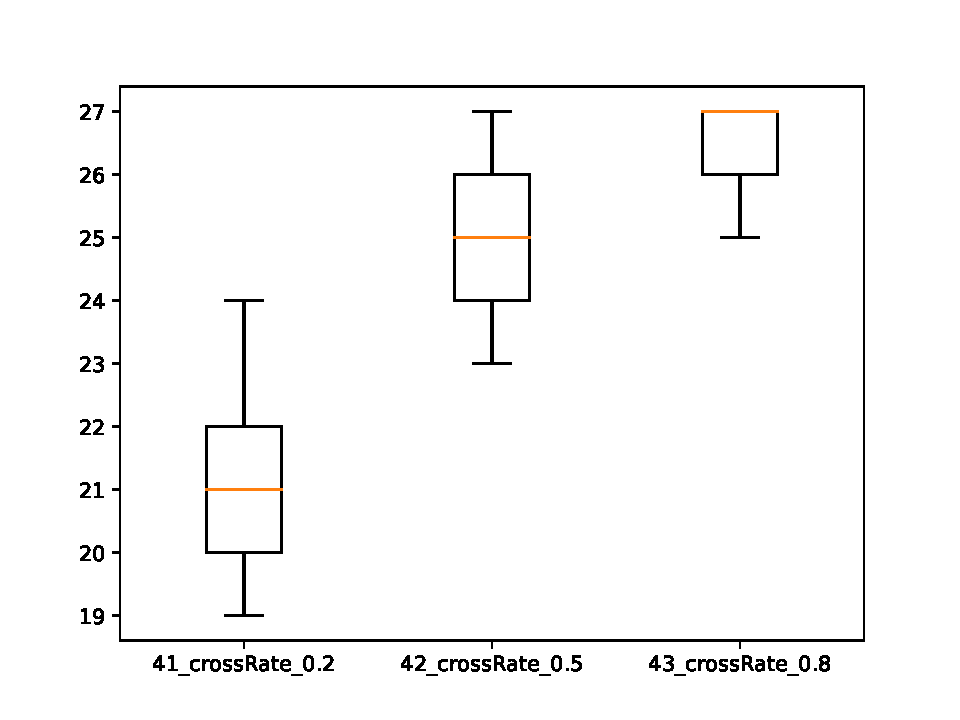
\includegraphics[scale=0.5]{teste4.pdf}
\end{minipage}
\end{minipage}


\subsection{Teste 4: Avaliação do efeito da probabilidade de mutação}




\end{document}